\documentclass[a4paper,12pt]{article}
\usepackage[utf8]{inputenc}
\usepackage[T2A]{fontenc}
\usepackage[russian]{babel}
\usepackage{amsmath, amsfonts, amssymb}
\usepackage{graphicx}
\usepackage{booktabs}
\usepackage{geometry}
\usepackage{float}
\usepackage{subcaption}
\usepackage{enumitem}
\usepackage{hyperref}
\geometry{left=2cm, right=2cm, top=2cm, bottom=2cm}
\graphicspath{{figures/}}
\hypersetup{colorlinks=true, linkcolor=blue, urlcolor=blue}
\setlist[itemize]{nosep, topsep=0.2em}
\setlist[enumerate]{nosep, topsep=0.2em}

\title{Лабораторная работа №2\\Продвинутые методы безусловной оптимизации}
\author{Команда: Егор Гуров, Александр Громоздин, Николай Гавришок}
\date{}

\begin{document}
\maketitle

\section*{Титульная информация}
\textbf{Вариант:} пакет оракулов и датасетов №2 (Logistic/ Poisson + $L_2$), исследовательский трек 4 (Cautious L-BFGS, отказ от Вульфа), невыпуклая 2D-функция Била.

\subsection*{Распределение ролей (согласно \texttt{README.md})}
\begin{description}
    \item[Егор Гуров] Аналитический вывод формул для Logistic/ Poisson и \texttt{hess\_vec}; проверка оракулов и разностных формул; математическая часть отчёта; теоретическое описание экспериментов 2.2--2.3; анализ трека~4.
    \item[Александр Громоздин] \texttt{LineSearchTool}, \texttt{linear\_conjugate\_gradients}, \texttt{nonlinear\_conjugate\_gradients}, \texttt{hessian\_free\_newton}; интеграция ноутбука и основных экспериментов; анализ на \textit{phishing} и \textit{real-sim}.
    \item[Николай Гавришок] \texttt{hess\_vec}, \texttt{hess\_vec\_finite\_diff}, \texttt{lbfgs}, \texttt{cautious\_lbfgs}; эксперименты 2.4--2.6 и трек~4; графики, таблицы, вёрстка \LaTeX-отчёта, PDF и презентации.
\end{description}
Замечание: распределение сделано примерно поровну; обязанности зафиксированы в \texttt{README.md}.

% --- Эксперимент 2.4
\section{Эксперимент 2.4. Сравнение методов на реальных ML-задачах}
\subsection*{Постановка (текст для отчёта)}
% TODO: сравнение Nonlinear CG, HFN, L-BFGS, GD, (полный Ньютон при умеренной размерности); критерий остановки; датасеты \textit{phishing}, \textit{cadata}, \textit{real-sim}.

\subsection*{Графики: значение функции от времени}
\begin{figure}[H]
  \centering
  \begin{subfigure}[b]{0.32\textwidth}
    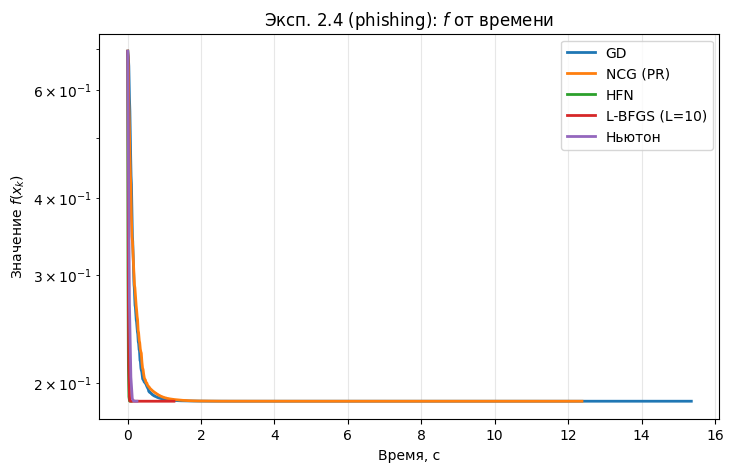
\includegraphics[width=\linewidth]{exp24_func_vs_time_phishing}
    \caption{\textit{phishing}}
  \end{subfigure}
  \hfill
  \begin{subfigure}[b]{0.32\textwidth}
    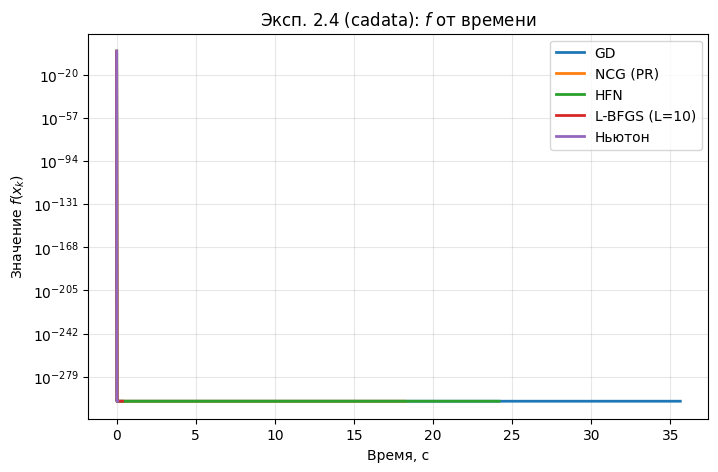
\includegraphics[width=\linewidth]{exp24_func_vs_time_cadata}
    \caption{\textit{cadata}}
  \end{subfigure}
  \hfill
  \begin{subfigure}[b]{0.32\textwidth}
    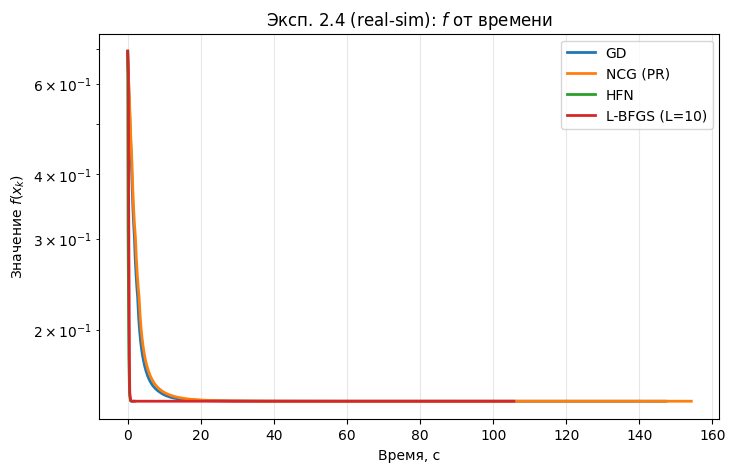
\includegraphics[width=\linewidth]{exp24_func_vs_time_real-sim}
    \caption{\textit{real-sim} ($n \gg m$)}
  \end{subfigure}
  \caption{Эксперимент 2.4: $f(x_k)$ от wall-clock времени (после запуска ноутбука с \texttt{real-sim} появятся PNG в \texttt{report/figures/}).}
\end{figure}

\subsection*{Графики: относительный квадрат нормы градиента от времени}
\begin{figure}[H]
  \centering
  \begin{subfigure}[b]{0.32\textwidth}
    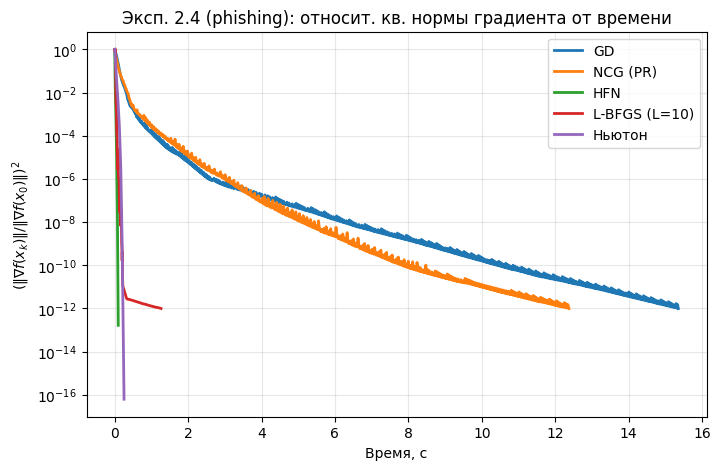
\includegraphics[width=\linewidth]{exp24_gradnorm_vs_time_phishing}
    \caption{\textit{phishing}}
  \end{subfigure}
  \hfill
  \begin{subfigure}[b]{0.32\textwidth}
    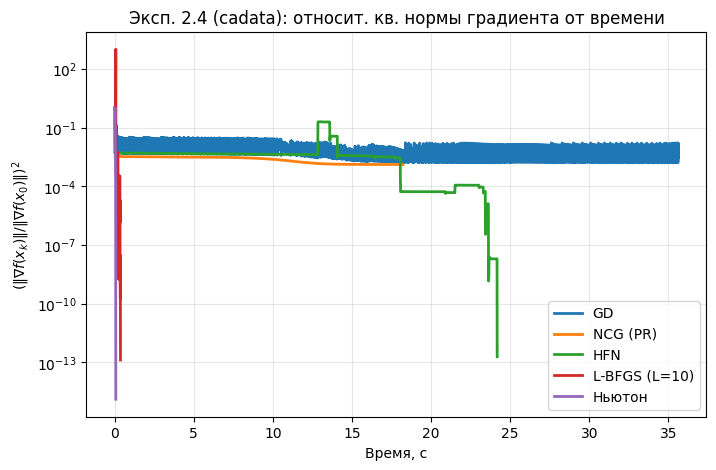
\includegraphics[width=\linewidth]{exp24_gradnorm_vs_time_cadata}
    \caption{\textit{cadata}}
  \end{subfigure}
  \hfill
  \begin{subfigure}[b]{0.32\textwidth}
    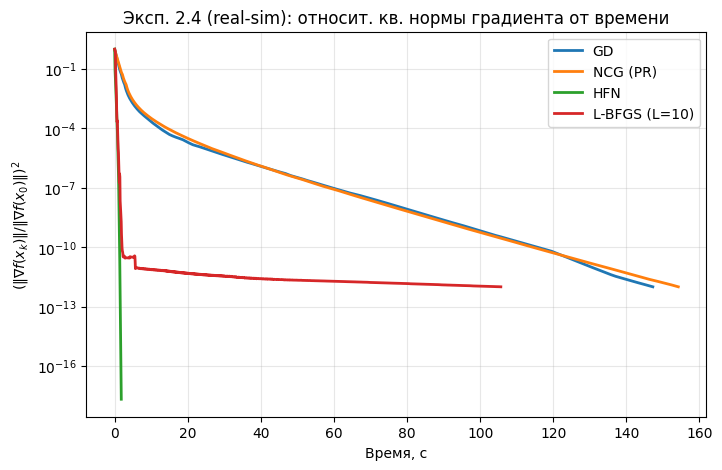
\includegraphics[width=\linewidth]{exp24_gradnorm_vs_time_real-sim}
    \caption{\textit{real-sim}}
  \end{subfigure}
  \caption{Эксперимент 2.4: $(\lVert \nabla f(x_k) \rVert / \lVert \nabla f(x_0) \rVert)^2$ от времени.}
\end{figure}

\subsection*{Сводная таблица (заполнить по результатам запуска)}
\begin{table}[H]
  \centering
  \begin{tabular}{@{}lrr@{}}
    \toprule
    Метод & Число внешних итераций & Время работы (с) \\
    \midrule
    \textit{phishing} && \\
    \midrule
    GD &  &  \\
    NCG (PR) &  &  \\
    HFN &  &  \\
    L-BFGS &  &  \\
    Ньютон (если применялся) &  &  \\
    \midrule
    \textit{cadata} && \\
    \midrule
    GD &  &  \\
    NCG (PR) &  &  \\
    HFN &  &  \\
    L-BFGS &  &  \\
    Ньютон (если применялся) &  &  \\
    \midrule
    \textit{real-sim} && \\
    \midrule
    GD &  &  \\
    NCG (PR) &  &  \\
    HFN &  &  \\
    L-BFGS &  &  \\
    Ньютон (при $n \ge 1000$ не запускается) & — & — \\
    \bottomrule
  \end{tabular}
  \caption{Эксперимент 2.4: сводка по датасетам. Уточнить числа по логу ноутбука.}
\end{table}

\subsection*{Выводы}
% TODO: текст

% --- Эксперимент 2.5
\newpage
\section{Эксперимент 2.5. Микропрофилирование}
\begin{figure}[H]
  \centering
  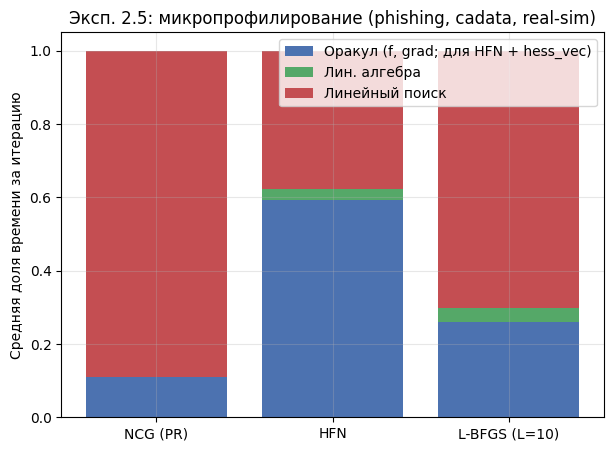
\includegraphics[width=0.75\textwidth]{exp25_microprofiling}
  \caption{Эксперимент 2.5: средние доли времени (оракул / линейная алгебра / линейный поиск) по итерациям для NCG, HFN, L-BFGS на датасетах п.~2.4.}
\end{figure}

\subsection*{Выводы}
% TODO: текст

% --- Эксперимент 2.6
\newpage
\section{Эксперимент 2.6. Оптимизация и качество на тесте}
\begin{figure}[H]
  \centering
  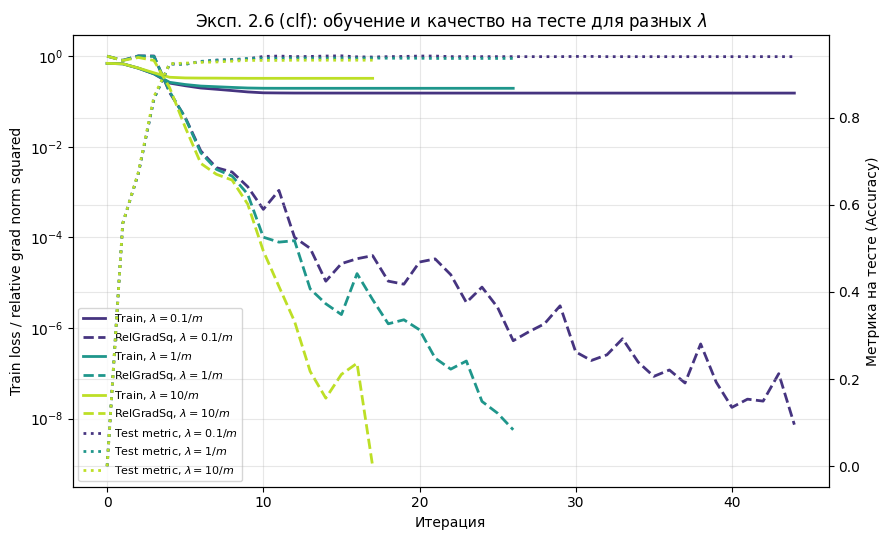
\includegraphics[width=0.88\textwidth]{exp26_train_vs_quality_clf}
  \caption{Классификация (\textit{phishing}): train loss, $\lVert \nabla f \rVert$, метрика на тесте (Accuracy).}
\end{figure}
\begin{figure}[H]
  \centering
  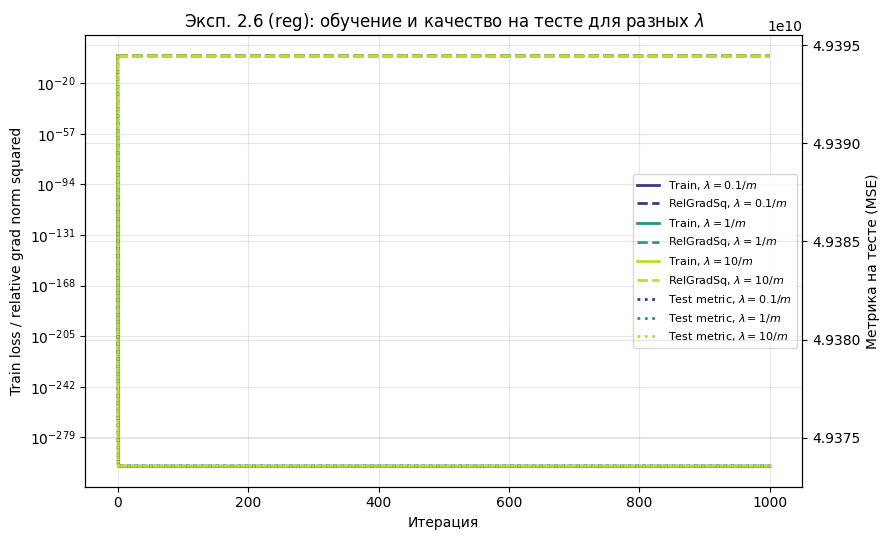
\includegraphics[width=0.88\textwidth]{exp26_train_vs_quality_reg}
  \caption{Регрессия (\textit{cadata}): аналогично, метрика на тесте (MSE).}
\end{figure}

\subsection*{Выводы}
% TODO: текст

% --- Трек 4
\newpage
\section{Исследовательский трек 4. Cautious L-BFGS и отказ от Вульфа}
Аппроксимация кривизны устойчива, если пары $(s_k, y_k)$ удовлетворяют (пример) условию
\begin{equation}
  \frac{\langle s_k, y_k \rangle}{\lVert s_k \rVert^2} > \varepsilon \lVert \nabla f(x_k) \rVert^\alpha
\end{equation}
(конкретные $\varepsilon$, $\alpha$ взяты из кода/методички). При нарушении — обновление истории BFGS пропускается.

\begin{figure}[H]
  \centering
  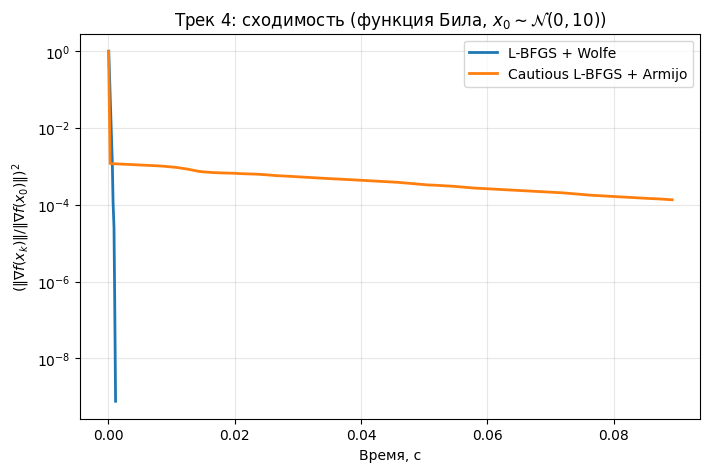
\includegraphics[width=0.85\textwidth]{track4_comparison}
  \caption{Трек~4, функция Била: относительный квадрат нормы градиента от времени, $x_0 \sim \mathcal{N}(0, 10)$ (по осям).}
\end{figure}

\begin{figure}[H]
  \centering
  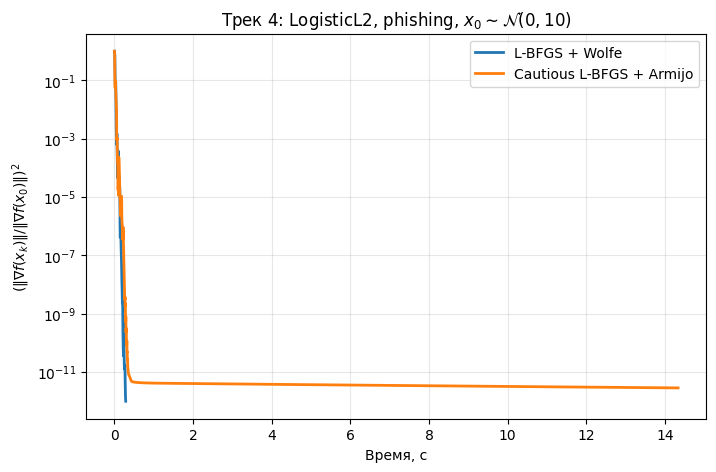
\includegraphics[width=0.85\textwidth]{track4_comparison_ml_phishing}
  \caption{Трек~4, \texttt{LogisticL2Oracle}, датасет \textit{phishing}, та же инициализация $x_0$; ось $X$ — время, $Y$ — относительный квадрат нормы градиента.}
\end{figure}

\begin{table}[H]
  \centering
  \small
  \begin{tabular}{@{}lrrrr@{}}
    \toprule
    Метод & Итераций & Средн.\ число вызовов оракула на ит. & Пропущ.\ обновлений памяти & Общее время (с) \\
    \midrule
    \multicolumn{5}{@{}l}{\emph{Функция Била}} \\
    L-BFGS + Wolfe &  &  &  &  \\
    Cautious L-BFGS + Armijo &  &  &  &  \\
    \midrule
    \multicolumn{5}{@{}l}{\emph{phishing, LogisticL2}} \\
    L-BFGS + Wolfe &  &  &  &  \\
    Cautious L-BFGS + Armijo &  &  &  &  \\
    \bottomrule
  \end{tabular}
  \caption{Трек~4: заполнить по логу ноутбука (средние вызовы: $(N_{\text{func}} + N_{\text{grad}}) / N_{\text{внеш. ит.}}$).}
\end{table}

\subsection*{Выводы}
% TODO: текст

\end{document}
